% Options for packages loaded elsewhere
\PassOptionsToPackage{unicode}{hyperref}
\PassOptionsToPackage{hyphens}{url}
\PassOptionsToPackage{dvipsnames,svgnames,x11names}{xcolor}
%
\documentclass[
  letterpaper,
  DIV=11,
  numbers=noendperiod]{scrartcl}

\usepackage{amsmath,amssymb}
\usepackage{iftex}
\ifPDFTeX
  \usepackage[T1]{fontenc}
  \usepackage[utf8]{inputenc}
  \usepackage{textcomp} % provide euro and other symbols
\else % if luatex or xetex
  \usepackage{unicode-math}
  \defaultfontfeatures{Scale=MatchLowercase}
  \defaultfontfeatures[\rmfamily]{Ligatures=TeX,Scale=1}
\fi
\usepackage{lmodern}
\ifPDFTeX\else  
    % xetex/luatex font selection
\fi
% Use upquote if available, for straight quotes in verbatim environments
\IfFileExists{upquote.sty}{\usepackage{upquote}}{}
\IfFileExists{microtype.sty}{% use microtype if available
  \usepackage[]{microtype}
  \UseMicrotypeSet[protrusion]{basicmath} % disable protrusion for tt fonts
}{}
\makeatletter
\@ifundefined{KOMAClassName}{% if non-KOMA class
  \IfFileExists{parskip.sty}{%
    \usepackage{parskip}
  }{% else
    \setlength{\parindent}{0pt}
    \setlength{\parskip}{6pt plus 2pt minus 1pt}}
}{% if KOMA class
  \KOMAoptions{parskip=half}}
\makeatother
\usepackage{xcolor}
\setlength{\emergencystretch}{3em} % prevent overfull lines
\setcounter{secnumdepth}{-\maxdimen} % remove section numbering
% Make \paragraph and \subparagraph free-standing
\ifx\paragraph\undefined\else
  \let\oldparagraph\paragraph
  \renewcommand{\paragraph}[1]{\oldparagraph{#1}\mbox{}}
\fi
\ifx\subparagraph\undefined\else
  \let\oldsubparagraph\subparagraph
  \renewcommand{\subparagraph}[1]{\oldsubparagraph{#1}\mbox{}}
\fi


\providecommand{\tightlist}{%
  \setlength{\itemsep}{0pt}\setlength{\parskip}{0pt}}\usepackage{longtable,booktabs,array}
\usepackage{calc} % for calculating minipage widths
% Correct order of tables after \paragraph or \subparagraph
\usepackage{etoolbox}
\makeatletter
\patchcmd\longtable{\par}{\if@noskipsec\mbox{}\fi\par}{}{}
\makeatother
% Allow footnotes in longtable head/foot
\IfFileExists{footnotehyper.sty}{\usepackage{footnotehyper}}{\usepackage{footnote}}
\makesavenoteenv{longtable}
\usepackage{graphicx}
\makeatletter
\def\maxwidth{\ifdim\Gin@nat@width>\linewidth\linewidth\else\Gin@nat@width\fi}
\def\maxheight{\ifdim\Gin@nat@height>\textheight\textheight\else\Gin@nat@height\fi}
\makeatother
% Scale images if necessary, so that they will not overflow the page
% margins by default, and it is still possible to overwrite the defaults
% using explicit options in \includegraphics[width, height, ...]{}
\setkeys{Gin}{width=\maxwidth,height=\maxheight,keepaspectratio}
% Set default figure placement to htbp
\makeatletter
\def\fps@figure{htbp}
\makeatother

\usepackage{algpseudocode}
\usepackage{algorithm}
\KOMAoption{captions}{tableheading}
\makeatletter
\makeatother
\makeatletter
\makeatother
\makeatletter
\@ifpackageloaded{caption}{}{\usepackage{caption}}
\AtBeginDocument{%
\ifdefined\contentsname
  \renewcommand*\contentsname{Table of contents}
\else
  \newcommand\contentsname{Table of contents}
\fi
\ifdefined\listfigurename
  \renewcommand*\listfigurename{List of Figures}
\else
  \newcommand\listfigurename{List of Figures}
\fi
\ifdefined\listtablename
  \renewcommand*\listtablename{List of Tables}
\else
  \newcommand\listtablename{List of Tables}
\fi
\ifdefined\figurename
  \renewcommand*\figurename{Figure}
\else
  \newcommand\figurename{Figure}
\fi
\ifdefined\tablename
  \renewcommand*\tablename{Table}
\else
  \newcommand\tablename{Table}
\fi
}
\@ifpackageloaded{float}{}{\usepackage{float}}
\floatstyle{ruled}
\@ifundefined{c@chapter}{\newfloat{codelisting}{h}{lop}}{\newfloat{codelisting}{h}{lop}[chapter]}
\floatname{codelisting}{Listing}
\newcommand*\listoflistings{\listof{codelisting}{List of Listings}}
\makeatother
\makeatletter
\@ifpackageloaded{caption}{}{\usepackage{caption}}
\@ifpackageloaded{subcaption}{}{\usepackage{subcaption}}
\makeatother
\makeatletter
\@ifpackageloaded{tcolorbox}{}{\usepackage[skins,breakable]{tcolorbox}}
\makeatother
\makeatletter
\@ifundefined{shadecolor}{\definecolor{shadecolor}{rgb}{.97, .97, .97}}
\makeatother
\makeatletter
\makeatother
\makeatletter
\makeatother
\makeatletter
\@ifpackageloaded{algorithm}{}{\usepackage{algorithm}}
\makeatother
\makeatletter
\@ifpackageloaded{algpseudocode}{}{\usepackage{algpseudocode}}
\makeatother
\ifLuaTeX
  \usepackage{selnolig}  % disable illegal ligatures
\fi
\IfFileExists{bookmark.sty}{\usepackage{bookmark}}{\usepackage{hyperref}}
\IfFileExists{xurl.sty}{\usepackage{xurl}}{} % add URL line breaks if available
\urlstyle{same} % disable monospaced font for URLs
\hypersetup{
  pdftitle={Metapops},
  colorlinks=true,
  linkcolor={blue},
  filecolor={Maroon},
  citecolor={Blue},
  urlcolor={Blue},
  pdfcreator={LaTeX via pandoc}}

\title{Metapops}
\author{}
\date{}

\begin{document}
\maketitle

\algblock{Input}{EndInput}
\algnotext{EndInput}
\algblock{Output}{EndOutput}
\algnotext{EndOutput}
\newcommand{\Desc}[2]{\State \makebox[2em][l]{#1}#2}
\renewcommand{\Return}{\State \textbf{return}~}
\newcommand{\Print}{\State \textbf{print}~}
\newcommand{\Break}{\State \textbf{break}}
\newcommand{\Continue}{\State \textbf{continue}}
\newcommand{\True}{\textbf{true}}
\newcommand{\False}{\textbf{false}}
\renewcommand{\And}{\textbf{and}~}
\newcommand{\Or}{\textbf{or}~}
\renewcommand{\Not}{\textbf{not}~}
\newcommand{\To}{\textbf{to}~}
\newcommand{\DownTo}{\textbf{downto}~}

\ifdefined\Shaded\renewenvironment{Shaded}{\begin{tcolorbox}[boxrule=0pt, enhanced, interior hidden, breakable, sharp corners, borderline west={3pt}{0pt}{shadecolor}, frame hidden]}{\end{tcolorbox}}\fi

\floatname{algorithm}{Algorithm}

\hypertarget{relaxing-the-homogeneous-mixing-assumption}{%
\subsubsection{Relaxing the homogeneous mixing
assumption}\label{relaxing-the-homogeneous-mixing-assumption}}

A fundamental assumption of the simple compartmental model presented in
\textbf{?@sec-Compartmental\_models} is that any susceptible individual
is equally likely to become infected by any of the infectious
individuals (at a rate proportional to the size of each compartment in
the population). However, real-world populations are not uniform in
their interactions (particularly on a scale like that of
\textbf{?@sec-Melb\_SIR}), and the assumption of homogeneous mixing can
be relaxed to produce more realistic models that demonstrate
heterogeneous mixing patterns.

\hypertarget{multi-patch-metapopulation-model}{%
\subsection{Multi Patch `Metapopulation'
Model}\label{multi-patch-metapopulation-model}}

In the simple SIR model of \textbf{?@sec-CompartmentalModels}, a single
population is divided into a number of compartments, each with their own
properties.

We can extend this model to instead consider a set of \(n\) populations,
each with their own number of residents \(N_i\) for that make up the
larger population \(N\)

\[
\sum\limits_{i=1}^{n}N_i = N
\]

Each of these sub-populations, which will hereafter be referred to as
`patches', contains compartments which behave analogously to those from
\textbf{?@sec-CompartmentalModels}, such that

\[ S_{i} + I_i + R_i = N_i \]

While individuals can only transition between compartments of their
respective patch (i.e.~\(N_i\) is constant), patches are coupled such
that susceptibles may still contract the disease by coming in to contact
with infectious individuals from another patch. The coupling between two
patches \(i,j \in \{1,\ldots, n\}\) is termed the mixing coefficient,
denoted \(m_{ij}\), and is defined as the probability that an individual
from patch \(i\) will next come into contact by an individual from patch
\(j\). As such, \(0 \leq m_{ij} \leq 1\) and \(\sum_j m_{ij} =1\).

We can now define the \texttt{force\ of\ infection} in patch \(i\) that
is exerted by infectious individuals from patch \(j\), as

\[
\lambda_{ij} = \beta \cdot I_j \cdot m_{i,j}
\]

The total force of infection experience by patch \(i\)

\[
\Lambda_i = \sum\limits_{j =1}^{n}\lambda_{ij}
\]

And thus describe an ODE model of patch \(i\) as

\[
\begin{aligned}
S'_{i} & =-\Lambda_i \cdot \frac{S_i}{N_i} \\
I'_{i} & =\Lambda_i \cdot \frac{S_i}{N_{i}}-\gamma I_i \\
R'_{i} & = \gamma I_i
\end{aligned}
\]

Similarly to \textbf{?@sec-Stochastic} SIR, we can construct a
Continuous Time Markov Chain Metapopulation SIR model with a state space

\begin{equation}\protect\hypertarget{eq-Metapopulation_CTMC_StateSpace}{}{\mathbb{S}=\left\{\left(s_1,  \ldots, s_i, \ldots, s_n, i_1,\ldots, i_i, \ldots , i_n\right): 0\geq s_i, i_i; s_i+i_i<N_j\right\}}\label{eq-Metapopulation_CTMC_StateSpace}\end{equation}

and transition rates

\begin{equation}\protect\hypertarget{eq-Meta_CTMC_rates}{}{
\begin{aligned}
q_{x, x+ inf_{i}} &=  \Lambda_i \frac{S_i}{N_{i}}\\
q_{x, x+ rec_{i}} &= \gamma I_i\end{aligned}
}\label{eq-Meta_CTMC_rates}\end{equation}

for \(i, j \in \{1,\ldots,n\}\), where

\begin{itemize}
\item
  \(x = \left(s_1, \ldots, s_i, \ldots, s_n, i_1,\ldots, i_i, \ldots , i_n\right)\)
\item
  \(\mathbf{inf}_{i}=\mathbf{e}_{2 i}-\mathbf{e}_{i}\), where
  \(\mathbf{e}_i\) is a vector of \(0\)s (length \(2n\)) with a \(1\) in
  the \(i^{\text {th }}\) position,
\item
  \(\mathbf{rec}_{i} = -\mathbf{e}_{2i}\)
\end{itemize}

Following from \textbf{?@sec-Stochastic\_SIR\_sim}, we can simulate
sample paths of this CTMC meta-population model using a stochastic
simulation algorithm
( Algorithm~\ref{alg-SIR_Metapopulation_Gillespie} ). The process
outlined in  Algorithm~\ref{alg-SIR_Metapopulation_Gillespie}  is
similar to that of  Algorithm~\ref{alg-SIR_Gillespie}  with the main
distinction{[}\^{}metapop2s-1{]} being that there are now \(2n\)
possible events (i.e.~an infection and recovery event for each patch).
Each element of the state change vector \(\mathbf{v}\) now encodes both
the location and type of an event

\[
\mathbf{v}_{i} = \begin{cases}
\mathbf{e}_{2i} - \mathbf{e}_{i} & \text{for} i \leq n \\
-\mathbf{e}_{2i}, & \text{for} i > n \\
\end{cases} 
\]

The propensity vector \(\mathbf{a}\) is similarly defined using the
rates form \(Q\) defined in Equation~\ref{eq-Meta_CTMC_rates} such that

\[
a_{i}  =  \begin{cases} \frac{S_i}{N_{i}} \Lambda_i & \text{for} i \leq n \\
\gamma I_{n-i} & \text{for} i > n
\end{cases} 
\]

Note that the event location and type are determined by the same random
number \(r_1\).

Also note that a the beginning of a simulation, all patches are composed
of entirely susceptible individuals. A number, \(I_0\), of individuals
in a randomly selected patch, \(\alpha\), become infected before initial
transition rates are computed.

\[
\begin{aligned}
S_i(0) & = \begin{cases}N_i & \text { if } i \neq \alpha \\
N_i-E_0 & \text { if } i=\alpha\end{cases} \\
I_i(0) & = \begin{cases}0 & \text { if } i \neq \alpha \\
I_0 & \text { if }  i=\alpha\end{cases} \\
\end{aligned}
\]

for \(i \in \{1, \ldots, n\}\) where
\(\alpha \sim \mathcal{U}\{1, r\}\).

\begin{algorithm}[htb!]
\caption{Stochastic simulation of SIR Metapopulation CTMC}
\textbf{Input:} $\mathbf{N}$, $I_0$, $\beta$, $\gamma$, $M$
\label{alg-SIR_Metapopulation_Gillespie}
\begin{algorithmic}[1]
\State $t \gets 0.0$ \Comment{Initialise time} 
\ForAll{i} \Comment{Initialise susceptibles}
\State $S_{i} \gets N_{i}$
\EndFor
\State Select $i \sim \mathcal{U}[1,n]$,  $I_{i} \gets I_0$                               \Comment{Seed infection}
\While{$I \geq 0$}
\ForAll{$i \in \{1, \ldots , n\}$}                                             
\State $a_{i} \gets \frac{S_{i}}{N_{i}} \cdot \sum\limits_{j = 1}^{n} \beta \cdot I_j \cdot M'_{j,i}$\Comment{Update Infection Rates}
\State $a_{n+i} \gets \gamma I_{i}$\Comment{Update Recovery Rates}
\State update $a_{net} = a_{net} + a_i + a_{n+i}$
\EndFor
\State generate two random numbers $r_1, r_2 \sim \mathcal{U}(0,1)$
\State select $\mu$ such that $\sum\limits_{j = 1}^{\mu} a_j \leq r_1 a_{net}$
\State compute $\tau \gets \frac{1}{a_{net}}\ln(\frac{1}{r_2})$
\State update $X \gets X + v_\mu$
\State set $t \gets t + \tau$
\EndWhile
\end{algorithmic}
\end{algorithm}

\hypertarget{example-origin-destination-spatial-metapopulation-model}{%
\subsection{Example: Origin-destination Spatial Metapopulation
model}\label{example-origin-destination-spatial-metapopulation-model}}

Following @moss2019, we will use as an example a meta-population model
of the Greater Melbourne region subdivided into 40 patches according to
the @2023AustralianStatisticalGeographya SA3 classification system. The
population of each patch along with its numeric SA identifier is given
in \textbf{?@sec-appendix1} and shown in Figure~\ref{fig-GMelbSA3Pop}

\begin{figure}

{\centering 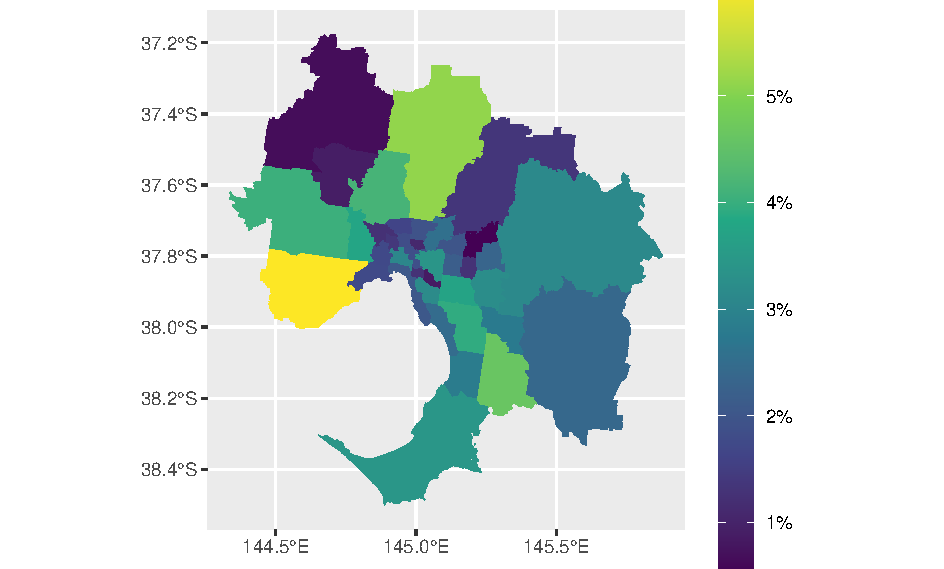
\includegraphics{metapop2s_files/figure-pdf/fig-GMelbSA3Pop-1.pdf}

}

\caption{\label{fig-GMelbSA3Pop}\textbf{?(caption)}}

\end{figure}

\hypertarget{origin-destination-mixing-matrix}{%
\subsubsection{Origin-destination mixing
matrix}\label{origin-destination-mixing-matrix}}

The mixing matrix was developed after @moss2019 using an empirically
informed origin-destination (OD) matrix derived from `Place of work'
data taken from the Australian Census @ABS\_census2016. Rows (`origin')
are the `usual residence', and the columns (destination) are the `place
of work'. The OD matrix

\[
F=\left(\begin{array}{cccc}f_{1,1} & f_{1,2} & \cdots & f_{1, n} \\f_{2,1} & f_{2,2} & \cdots & f_{2, n} \\ \vdots & \vdots & \ddots & \vdots \\f_{n, 1} & f_{n, 2} & \cdots & f_{n, n}\end{array}\right)
\]

\(f_{ij}\) is the proportion of people why usually reside in patch \(i\)
listing patch \(j\) as their place of work. This empirical method is
expected to describe contact patterns \emph{between regions}, but
contact patterns within \emph{within} the region of residence are
expected to result more from contact outside of a work
context.Therefore, diagonal elements are set to zero.

\[
\begin{aligned}
f_{i, i} & =0 \\
\sum_{j=1}^{r} f_{i, j} & =1 \quad \forall i \in [1 . . r]
\end{aligned}
\]

The final mixing matrix is defined using the `local' mixing is given by
a parameter \(\delta^H\). Diagonal elements are set to \(\delta^H\) with
the remaining proportion, \(\delta^* = 1-\delta^H_i\) distributed among
the non-local patches equally.

\[
M=\left(\begin{array}{cccc}
\delta_{1}^{H} & \delta_{1}^{*} f_{1,2} & \cdots & \delta_{1}^{*} f_{1, r} \\
\delta_{2}^{*} f_{2,1} & \delta_{2}^{H} & \cdots & \delta_{2}^{*} f_{2, r} \\
\vdots & \vdots & \ddots & \vdots \\
\delta_{r}^{*} f_{r, 1} & \delta_{r}^{*} f_{r, 2} & \cdots & \delta_{r}^{H}
\end{array}\right)
\]

OD matrices for several values of \(\delta^H\) are presented as heatmaps
in \textbf{?@fig-OD\_matrices}

\begin{figure}

\begin{minipage}[t]{0.50\linewidth}

{\centering 

\raisebox{-\height}{

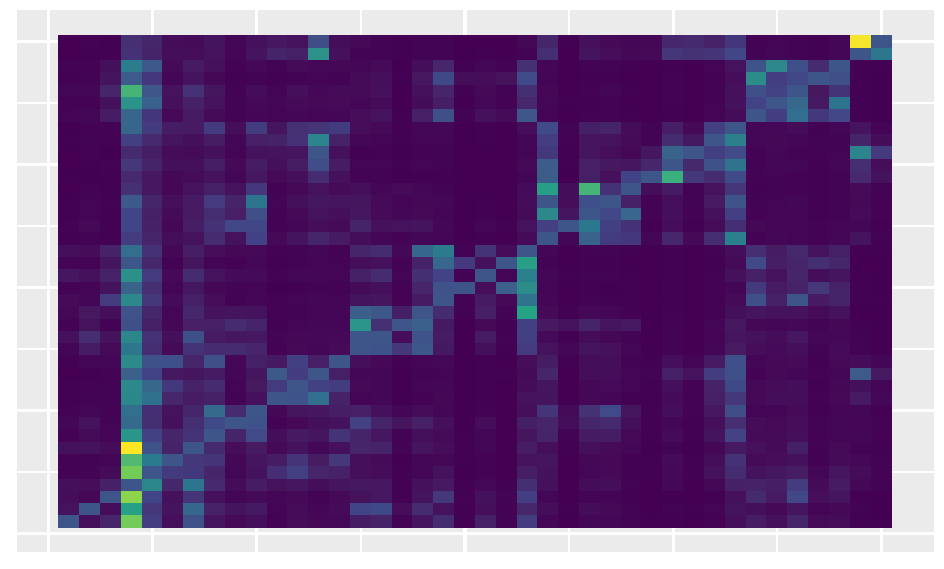
\includegraphics{metapop2s_files/figure-pdf/fig-SA3_OD_Mixmats-1.pdf}

}

}

\subcaption{\label{fig-SA3_OD_Mixmats-1}}
\end{minipage}%
%
\begin{minipage}[t]{0.50\linewidth}

{\centering 

\raisebox{-\height}{

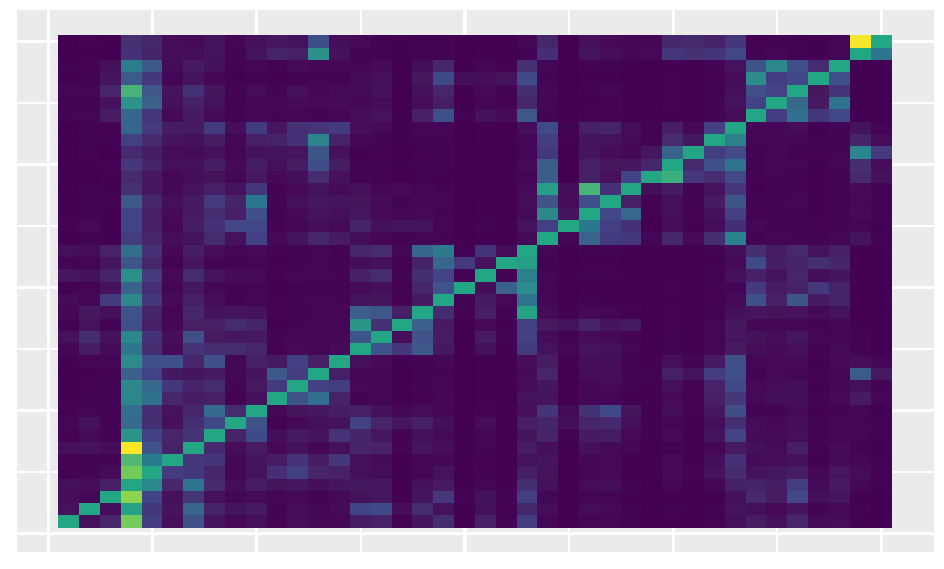
\includegraphics{metapop2s_files/figure-pdf/fig-SA3_OD_Mixmats-2.pdf}

}

}

\subcaption{\label{fig-SA3_OD_Mixmats-2}}
\end{minipage}%
\newline
\begin{minipage}[t]{0.50\linewidth}

{\centering 

\raisebox{-\height}{

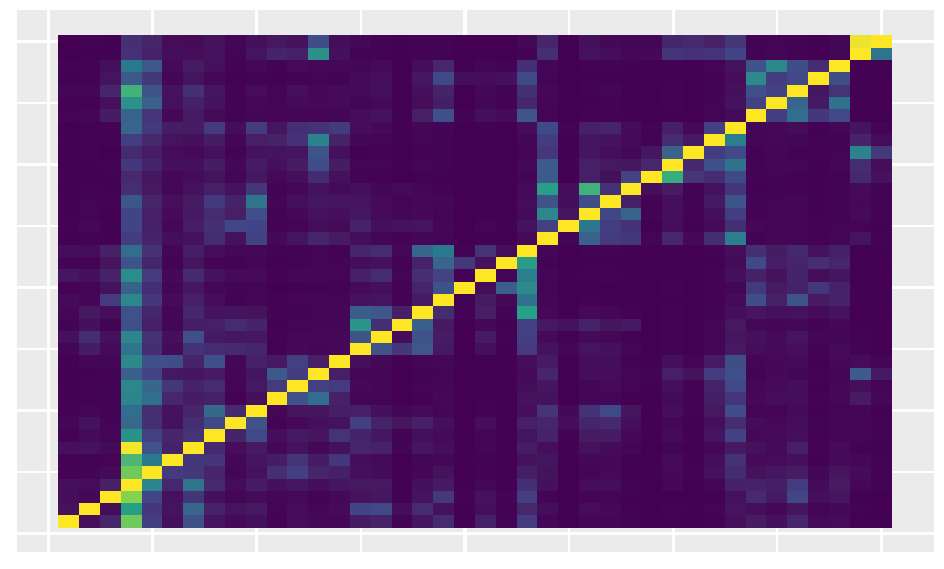
\includegraphics{metapop2s_files/figure-pdf/fig-SA3_OD_Mixmats-3.pdf}

}

}

\subcaption{\label{fig-SA3_OD_Mixmats-3}}
\end{minipage}%
%
\begin{minipage}[t]{0.50\linewidth}

{\centering 

\raisebox{-\height}{

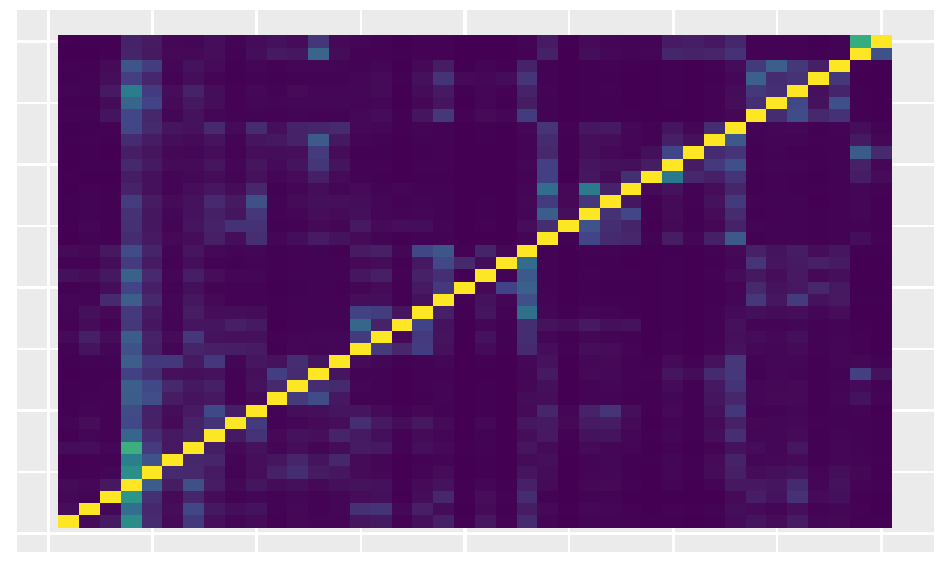
\includegraphics{metapop2s_files/figure-pdf/fig-SA3_OD_Mixmats-4.pdf}

}

}

\subcaption{\label{fig-SA3_OD_Mixmats-4}}
\end{minipage}%

\caption{\label{fig-SA3_OD_Mixmats}showing OD mixing matrices with
values of \(\delta^H\) = (a) 0.1, (b) 0.2, (c) 0.3, (d) 0.4}

\end{figure}

\hypertarget{simulation-results}{%
\subsubsection{Simulation results}\label{simulation-results}}

We can observe the metapopulation infection curves for our OD model for
a range of \(R_0\) and \(\delta^H\) values in
Figure~\ref{fig-SA3_OD_total_inf}, and the key infecton statistics in
Figure~\ref{fig-SA3_OD_outcomes}

\begin{figure}

{\centering 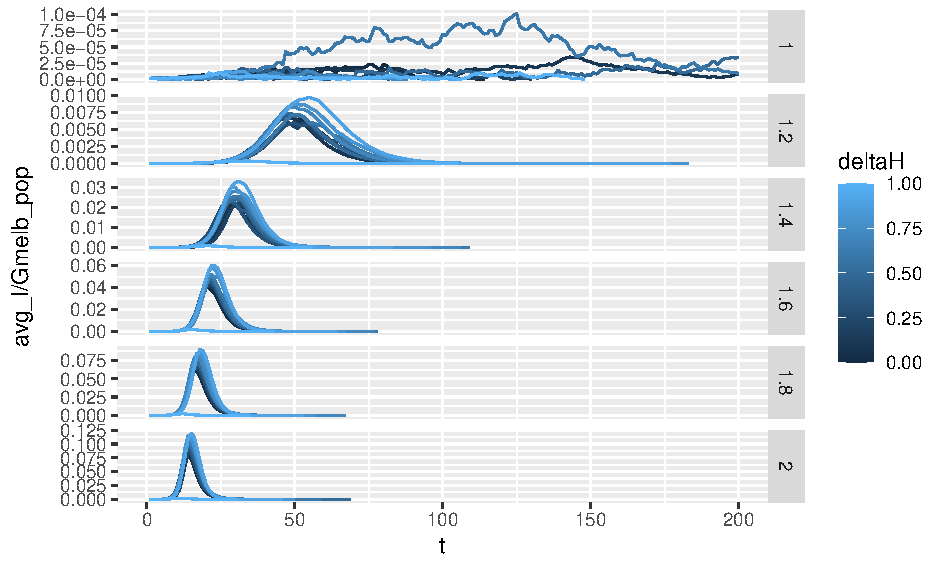
\includegraphics{metapop2s_files/figure-pdf/fig-SA3_OD_total_inf-1.pdf}

}

\caption{\label{fig-SA3_OD_total_inf}Average proportion of the
population over time for simulations of a OD mixing metapopulation model
of the melbourne metropolitan area with a range of Basic reproduction
numbers (\(R_0\)), and local mixing coefficients(\(\\delta^H\)). Note
the different y scale in each facet.}

\end{figure}

\begin{figure}

\begin{minipage}[t]{0.50\linewidth}

{\centering 

\raisebox{-\height}{

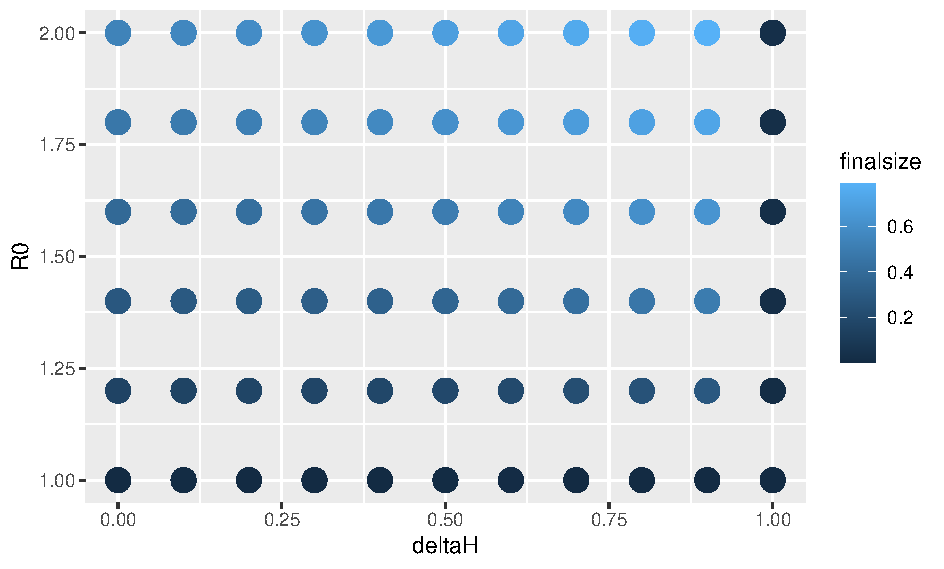
\includegraphics{metapop2s_files/figure-pdf/fig-SA3_OD_outcomes-1.pdf}

}

}

\subcaption{\label{fig-SA3_OD_outcomes-1}}
\end{minipage}%
%
\begin{minipage}[t]{0.50\linewidth}

{\centering 

\raisebox{-\height}{

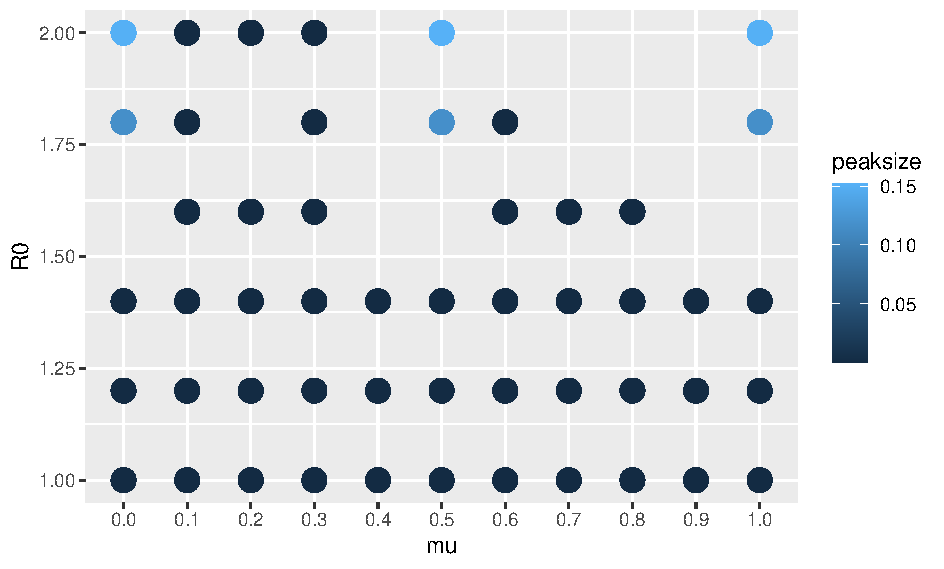
\includegraphics{metapop2s_files/figure-pdf/fig-SA3_OD_outcomes-2.pdf}

}

}

\subcaption{\label{fig-SA3_OD_outcomes-2}}
\end{minipage}%
\newline
\begin{minipage}[t]{0.50\linewidth}

{\centering 

\raisebox{-\height}{

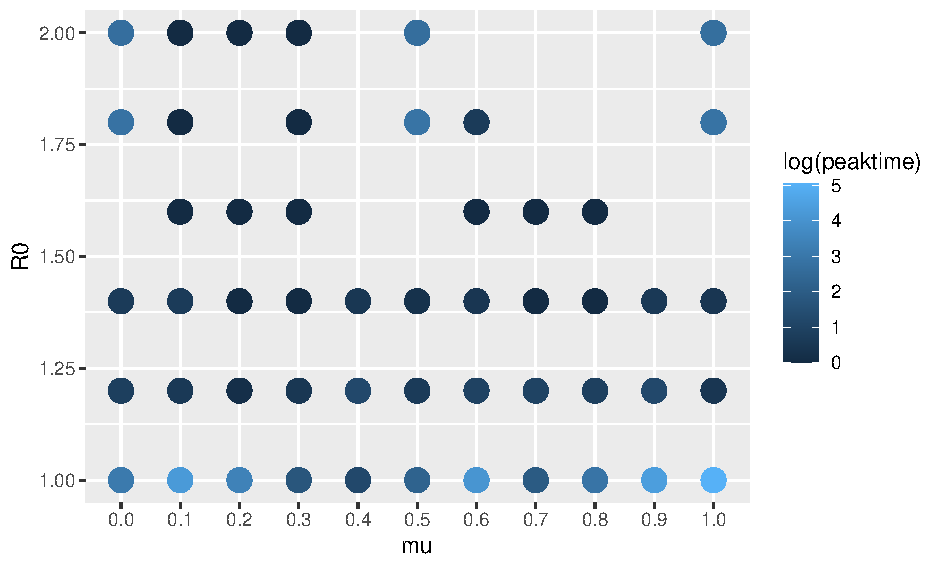
\includegraphics{metapop2s_files/figure-pdf/fig-SA3_OD_outcomes-3.pdf}

}

}

\subcaption{\label{fig-SA3_OD_outcomes-3}}
\end{minipage}%
%
\begin{minipage}[t]{0.50\linewidth}

{\centering 

\raisebox{-\height}{

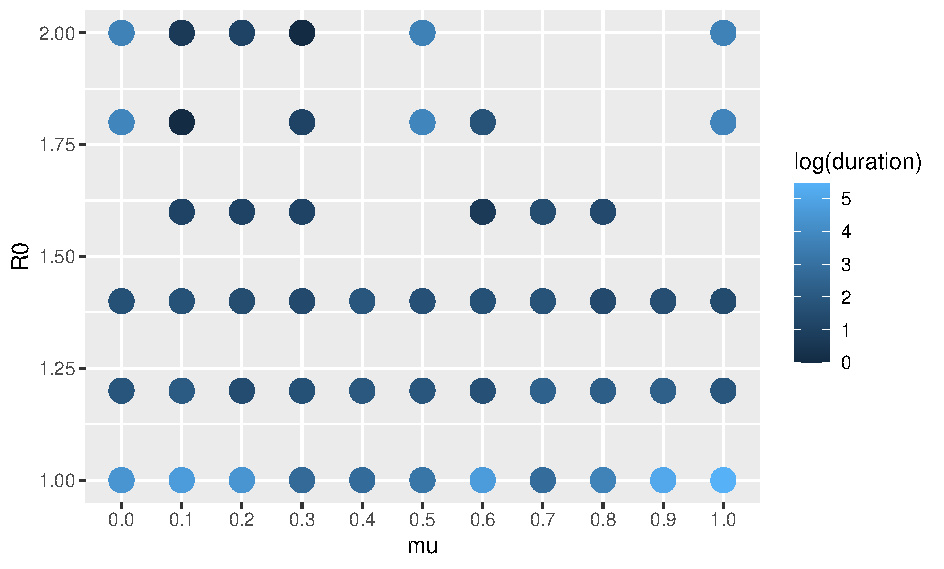
\includegraphics{metapop2s_files/figure-pdf/fig-SA3_OD_outcomes-4.pdf}

}

}

\subcaption{\label{fig-SA3_OD_outcomes-4}}
\end{minipage}%

\caption{\label{fig-SA3_OD_outcomes}Final (a) and peak (b) infection
numbers (as a proportion of the entire population), peak time (c) and
total duration (d) of a simulated SIR metapopulation model with OD
mixing matrix at different values of \(\delta^H\) and \(R_0\)}

\end{figure}

However, now we can decompose these metapopulation scale outcomes into
those of the underlying subpopulation. For example,
\textbf{?@fig-OD\_patchinf\_curve\_eg}

\begin{figure}

{\centering 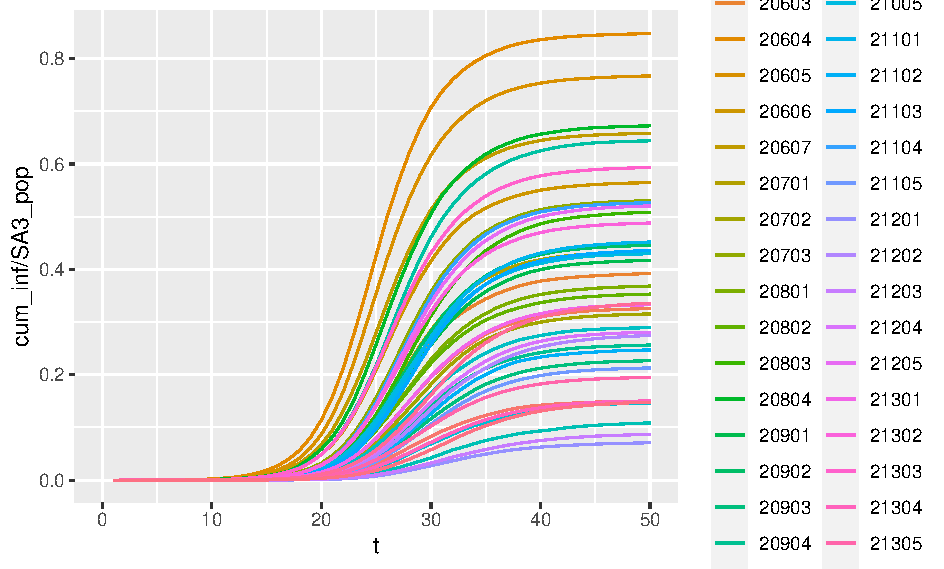
\includegraphics{metapop2s_files/figure-pdf/fig-SA3_OD_patchinf_curve_eg-1.pdf}

}

\caption{\label{fig-SA3_OD_patchinf_curve_eg}Cumulative infections (as a
proportion of patch population) for each SA3 scale patch in the first 50
days of single simulation of an OD mixing metapopulation SIR model of
the greater Melbourne region. \(R_0 = 1.4\), \(\delta^H = 0.5\).}

\end{figure}

And we can summarise over multiple simulations to get a better
understanding of the differential influence of the local mixing
parameter \(\delta ^H\) in each SA3 population. For example,
Figure~\ref{fig-SA3_OD_patch_peaks} shows the consistent trend toward
higher peak infections with greater proportons of local mixing (higher
\(\delta^H\)). However, certain patches demonstrate the opposite effect
- the Melbourne City patch for example has the highest peak proportion
infection (of any patch) when local mixing is low. This can be explained
by the relatively large number of residents from all patches working in
the city (this is evident in the OD mixing matrices of
Figure~\ref{fig-SA3_OD_Mixmats}, where the city POW is identifiable as a
bright column). High inter-patch mixing means that the city center has a
constant supply of infectious contacts.

\begin{figure}

{\centering 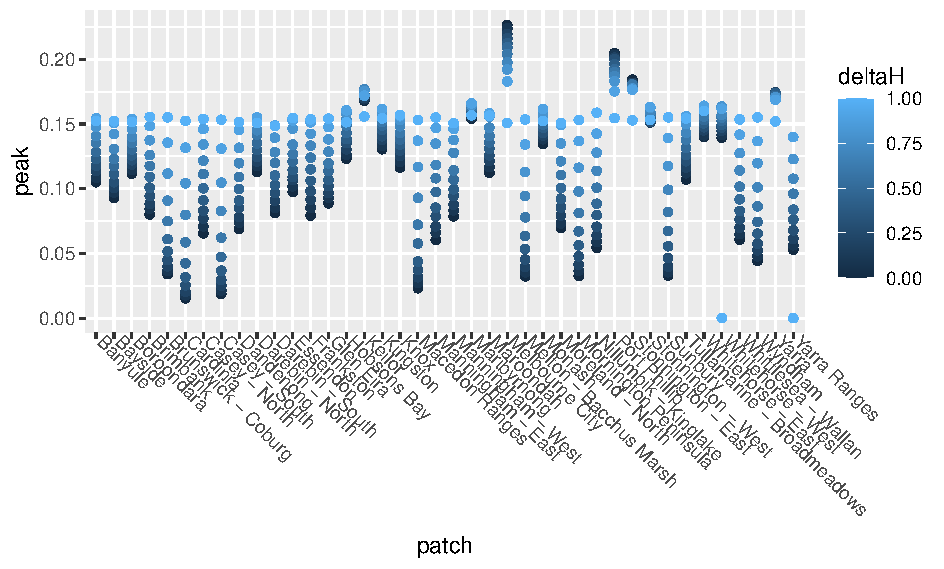
\includegraphics{metapop2s_files/figure-pdf/fig-SA3_OD_patch_peaks-1.pdf}

}

\caption{\label{fig-SA3_OD_patch_peaks}showing the peak proportion of
infected individuals in each SA3 patch of an OD mixing metapopulation
with varying contributions of local mixing(\delta\^{}H)}

\end{figure}



\end{document}
